\section{The Colombian Andean Bandola and its analysis}

Colombian Andean Bandola is a plucked string instrument that comes from guitar family. Its name comes from an old persian-arabic root, pandur, that comes through different north african and european instruments and indicates a variety of melodic instruments with high and medium pitch. This instrument presents several design adaptations through history in different Colombian regions that differ essentially in dimensions, process of building and tuning. Bandola in C (tuned in C) and bandola in B$\flat$ (tuned in B$\flat$) are the most representative prototypes.

The analysis proposed in this document is considered for bandola in C, which has been accepted and markedly used in last years by \textit{estudiantinas} (musical groups similar to Tunas). Hence, following descriptions pertain to this instrument with C-tuning. The bandola in C presents twelve strings grouped in unison pairs. Strings form six groups tuned in intervals of perfect fourths \cite{thesis:bandola}. Figure \ref{Bandola} presents the bandola and the pitchs for each string. The frequency values that correspond to the tuning of each open string are specified in Table \ref{StringTuning}.

\begin{figure}[h]
\centering
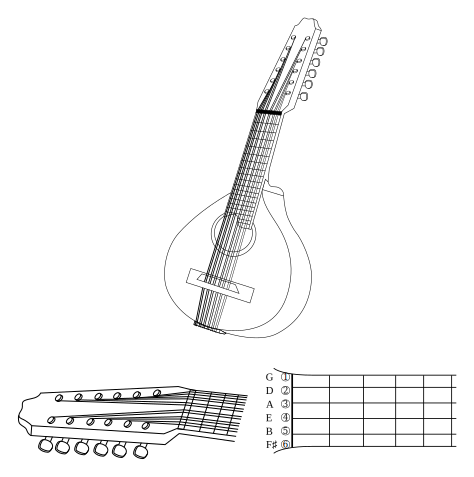
\includegraphics[height=5cm]{img/bandola.png}
\caption[Description of a Colombian Andean Bandola]{Upper image: Colombian Andean Bandola. Lower image: Pitch for each string. From top to bottom in fingerboard strings are tuned in: G, D, A, E, B, F$\sharp$}
\label{Bandola}
\end{figure}

\begin{table}[htb]
\centering
\begin{tabular}{|c|c|c|c|c|c|c|}\hline
\multicolumn{7}{|c|}{\vphantom{\LARGE Ap} Frequencies of tuning for the open strings}\\ \hline\hline
 & G4& D4 & A3 & E3 & B2 & F$\sharp$ 2\\ \hline
Hz & 783.99 & 587.33 & 440 & 329.63 & 246.94 & 185 \\ \hline
\end{tabular}
\caption{Frequency values that correspond to the tuning of open strings in the C-Bandola}
\label{StringTuning}
\end{table}  

Sources of sound in instruments could be of mechanical, acoustical or electrical type. For instance, vibrations of strings, bars, membranes, plates, air in a tube and synthesized sounds. Even sources could be collective coupled vibrators, in other words, a complex system \cite{Rossing}. Related to this fact, instrument analysis is classified according the type of source or sound production. This will indicate the phenomenon involved in each case, and thus, the useful mathematical formulation.

String instruments are a particular case of classification, which commonly, not only involve string vibration in an instrument, but also coupled plates, bars and air oscillations. Violins, guitars and bandola in C are examples in this category and many works have been devoted, at least for violins and guitars, to study their behavior as complex system \cite{Rossing,Christensen, Christensen3, Caldersmith1, Dickens1, Firth1}.

For simplicity, complex systems are divided in subsystems. As an exponent, the phenomena involved in guitars sound production will be presented to distinguish two main subsystems: the first composed by strings, bridge and top plate and the second composed by guitar body parts. Due to the great similarity of guitar and bandola, this example constitutes an excellent description to illustrate physical behavior of bandola in C.

In Figure \ref{GuitarScheme}, a scheme similar to one presented in \cite{Rossing} shows the frequency range in which each subsystem play significant role. From this figure, guitar behavior can be described  as follows: At low frequency, guitar transmits vibrations through the bridge to the top plate, which displaces fluid inside the cavity and induces pressure changes that cause sound hole radiation. Vibrational energy is also transmitted to back plate via both the ribs and air cavity pressure changes. At high frequency, most of the sound is radiated by top plate and the role of the bridge becomes more relevant.  

\begin{figure}[h]
\centering
\includegraphics[height=4cm]{img/GuitarScheme.png}
\caption{Scheme of guitar subsystems according to frequency response}
\label{GuitarScheme}
\end{figure}

This work will treat specifically the analysis of modal coupling at low resonances in the C-Bandola body and hence, the coupling between plates and the enclosed air. 